\chapter {Normalizacja odpowiedzi skokowych}

\section{Znormalizowane odpowiedzi}

W celu przekształcenia odpowiedzi skokowych do postaci używanych w algorytmie DMC dokanono ich normalizacji, analogicznie jak w pierwszym projekcie, tj. odjęto wartość w punkcie pracy i podzielono przez rozmiar skoku. Do wyznaczenia odpowiedzi toru sterowanie-wyjście użyto skoku wartości o 40 (tej samej co w poprzednim projekcie), natomiast dla toru zakłócenie-wyjście użyto skoku o 20. Obie znormalizowane odpowiedzi (dla skoku wartości w chwili k=0)  przedstawiono na rysunku \ref{normal_odp}:


\begin{figure}[h!]
	\centering
	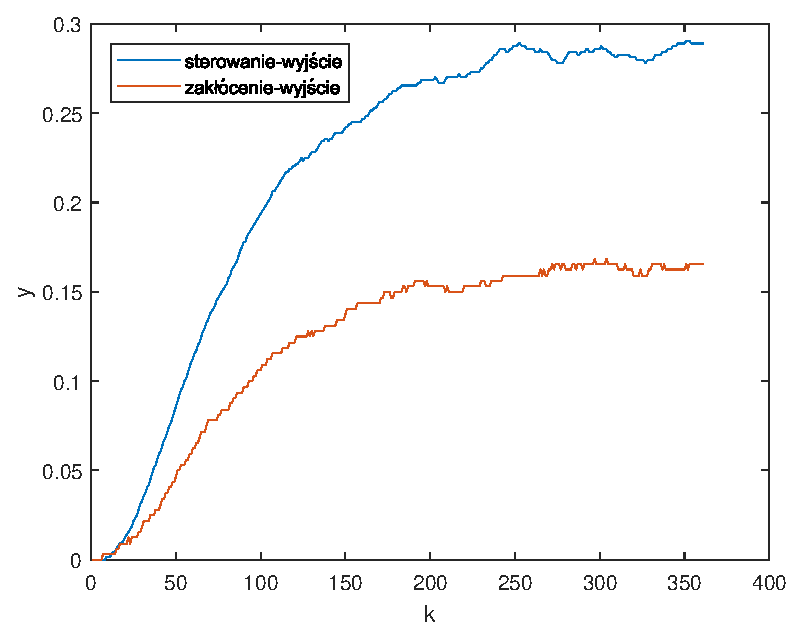
\includegraphics[scale=1]{Rys/LAB2_NormalStepResponses_Z3.eps}
	\caption{Znormalizowane odpowiedzi skokowe}
	\label{normal_odp}
\end{figure}


Ponieważ oba sygnały są wariacją jednego, tego samego sygnału dobrano dla nich taki sam horyzont dynamiki równy 361 (wyznaczony jako punkt w której wartość odpowiedzi po raz pierwszy przekracza 0,995 maksymalnej wartości).
\FloatBarrier

\section{Aproksymacja odpowiedzi skokowych}

W celu wygładzenia odpowiedzi skokowych dokonano ich aproksymacji jako dyskretnych członów inercyjnych drugiego rzędu z opóźnieniem tj.:

\begin{equation}
G(z)= \frac {z-1}{z} Z [\frac{K}{(sT_{1}+1)(sT_{2}+1)}e^{-T_{d}s}*\frac{1}{s}]
\label{wzor_0}
\end{equation}

Ogólna postać transmitancji w dziedzinie czasu dyskretnego ma postać:

\begin{equation}
G(z)= \frac{b_{1}z^{-1}+b_{2}z^{-2}} {1+a_{1}z^{-1}+a_{2}z^{-2}}z^{-T_{d}}
\label{wzor_1}
\end{equation}

Co przekłada się na następującą postać równania różnicowego:

\begin{equation}
y(k)=b_{1}u(k-T_{D}-1)+b_{2}u(k-T_{D}-2)-a_{1}y(k-1)-a_{2}y(k-2)
\label{wzor_2}
\end{equation}


Ponieważ wartości parametrów w tych wzorze wyrażają się poprzez $T_{1}, T_{2},K, T_{d}$ właśnie te zmienne optymalizowano. Użyto do tego skryptów \verb|Optymalizacja_LAB2.m| oraz \verb approx_error.m, zawierające funkcje fmincon, optymalizujące parametry, gdzie jedyne więzy narzucono na całkowitą i nieujemną wartość $T_{d}$.  Rezultaty przedstawiono na rysunkach \ref{wej_odp} i \ref{zak_odp}:



\begin{figure}[h!]
	\centering
	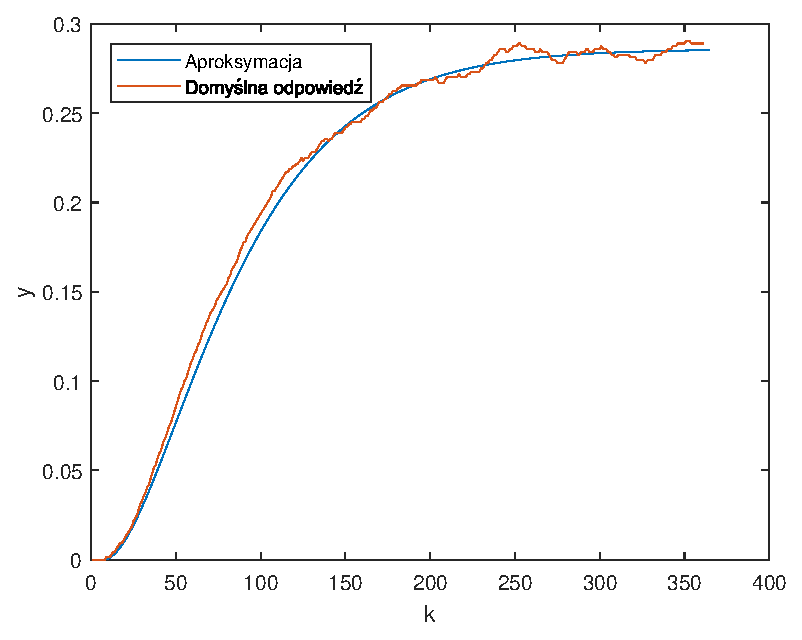
\includegraphics[scale=1]{Rys/LAB12_AproxedY.eps}
	\caption{Aproksymacja toru sterowanie-wyjście}
	\label{wej_odp}
\end{figure}

\begin{figure}[h!]
	\centering
	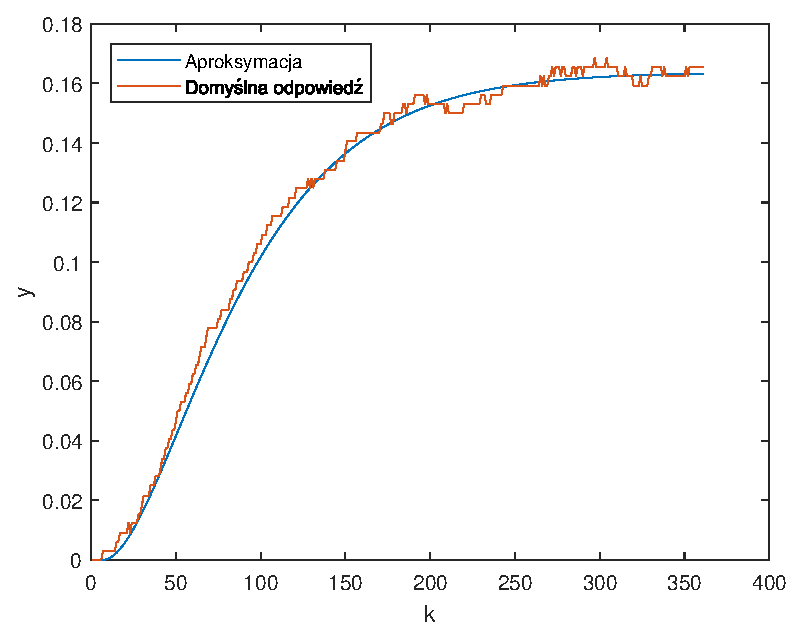
\includegraphics[scale=1]{Rys/LAB12_AproxedZ.eps}
	\caption{Aproksymacja toru zakłócenie-wyjście}
	\label{zak_odp}
\end{figure}
\FloatBarrier


\FloatBarrier

Transmitancja toru sterowanie-wyjscie:

\begin{equation}
G(z)= \frac{7,799*10^{-5}z^{-1}+7,678*10^{-5}z^{-2}} {1-1,953z^{-1}+0,954z^{-2}}z^{-3}
\label{wzor_11}
\end{equation}

Transmitancja toru zakłócenie-wyjscie:

\begin{equation}
G(z)= \frac{3,955*10^{-5}z^{-1}+3,898*10^{-5}z^{-2}} {1-1,957z^{-1}+0,957z^{-2}}z^{-3}
\label{wzor_12}
\end{equation}


